\documentclass[a4paper,10pt]{article}
\usepackage[paper=a4paper, hmargin=1.5cm, bottom=1.5cm, top=3.5cm]{geometry}
\usepackage[latin1]{inputenc}
\usepackage[T1]{fontenc}
\usepackage[spanish]{babel}
\usepackage{amssymb}
\usepackage{amsmath}
\usepackage{mathtools}
\usepackage{fancyhdr}
\usepackage{lastpage}
\usepackage{caratula}
\usepackage{verbatim}
\usepackage{xspace}
\usepackage{xargs}
\usepackage{float}
\usepackage{graphicx}
\usepackage{ifthen}
\usepackage[spanish,noline,longend]{algorithm2e}
\usepackage{listings}
\usepackage{braket}
%\usepackage{aed2-tad,aed2-symb,aed2-itef}

\lstset{language=C++, tabsize=4, breaklines=true, breakatwhitespace=true, numbers=left, numbersep=10pt}




\pagestyle{fancy}
\thispagestyle{fancy}
\addtolength{\headheight}{1pt}
\cfoot{\thepage /\pageref{LastPage}}
\renewcommand{\footrulewidth}{0.4pt}


\begin{document}


\begin{center}
\begin{Large}
\textbf{Resumen Organizaci\'on del Computador II}
\end{Large}
\end{center}
\begin{center}
Axel Straminsky
\end{center}


\begin{center}
Diciembre 2014
\end{center}

\vspace*{11\baselineskip}


\begin{center}
\begin{figure}[htb]
\begin{center}

\includegraphics[width=8cm]{./logo_uba}
\end{center}
\end{figure}
\end{center}


\begin{center}
\begin{figure}[htb]
\begin{center}

\includegraphics[width=8cm]{./logo_dc}
\end{center}
\end{figure}
\end{center}



\vspace*{8\baselineskip}


Aclaraci\'on: Este apunte es un resumen que use para preparar el final de Orga 2. El apunte no est\'a completo, es decir, no abarca el total
de la materia, ni necesariamente est\'a del todo correcto.

\newpage

\tableofcontents

\newpage
\section{Procesos}
\subsection{Introduccion}

Un proceso es una abstracción de un programa en ejecución, que básicamente convierte una CPU en varias CPU virtuales, proporcionando de esta manera la capacidad de operar (pseudo)concurrentemente, incluso cuando hay una sola CPU disponible.

Un proceso no es más que una instancia de un programa en ejecución, incluyendo los valores actuales del contador de programa, los registros y las variables. En concepto, cada proceso tiene su propia CPU virtual; en la realidad, la CPU real conmuta de un proceso a otro. Varios procesos pueden compartir un solo procesador mediante el uso de un algoritmo de planificación para determinar cuándo se debe detener el trabajo en un proceso para dar servicio a otro.

Hay cuatro eventos principales que provocan la creación de procesos:
\begin{itemize}
\item El arranque del sistema
\item La ejecución de una llamada al sistema para creación de procesos.
\item Una petición de usuario para crear un proceso.
\item El inicio de un trabajo por lotes.
\end{itemize}

Algunos procesos corren en primer plano, es decir, interactúan con los usuarios, mientras que otros procesos, que no están asociados con usuarios específicos sino con una función específica, corren en segundo plano. Un ejemplo sería un proceso que acepte peticiones entrantes para las páginas web hospedadas en ese equipo; estos procesos se conocen como \textbf{daemons}.

En UNIX sólo hay una llamada al sistema para crear un proceso: \textbf{fork}. Esta llamada crea un clon exacto del proceso que hizo la llamada. Después del fork, los dos procesos (padre e hijo) tienen la misma imagen de memoria, las mismas variables de entorno y los mismos archivos abiertos. Por lo general, el proceso hijo ejecuta después a \textbf{execve} o una llamada al sistema similar para cambiar su imagen de memoria y ejecutar un nuevo programa. La razón de este proceso de dos pasos es para permitir al hijo manipular sus descriptores de archivo después de fork, pero antes de execve, para poder lograr la redirección de la entrada, salida y error estándar.

\subsection{Estados de un proceso}

Un proceso se puede encontrar en uno de tres estados:

\begin{itemize}
\item En ejecución (está usando la CPU en ese instante)
\item Listo (ejecutable. Se detuvo temporalmente para dejar que se ejecute otro proceso.)
\item Bloqueado (no puede ejecutarse hasta que ocurra cierto evento externo)
\end{itemize}

~\\
\begin{figure}[h]
	\begin{center}
	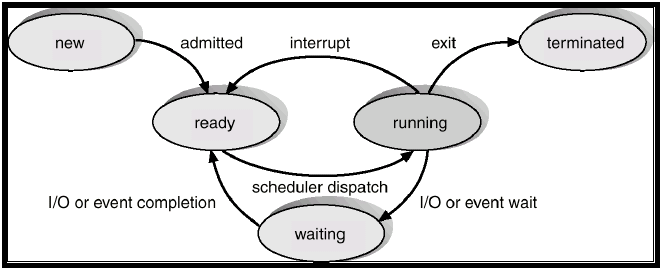
\includegraphics[width=0.8\textwidth]{imagenes/processstates.png}
	\caption{Estados de un proceso}
	\end{center}
\end{figure}
~\\

\subsection{Implementación de los procesos}

Para implementar el modelo de procesos, el SO mantiene una tabla llamada tabla de procesos, con una entrada por cada proceso (llamada Process Control Block (PCB)). Esta entrada contiene información importante acerca del estado de cada proceso, como el Program Counter, el Stack Pointer, asignación de memoria, estado de sus archivos abiertos, información para el scheduler, registros de la CPU, etc.

Cuando ocurre una interrupción, el PC, el PSW, y uno o más registros se meten en la pila mediante el hardware de interrupción. Después, la CPU salta a la dirección especificada en el vector de interrupción. Esto es todo lo que hace el hardware, en adelante es todo responsabilidad del software.

Todas las interrupciones comienzan por guardar los registros, a menudo en la entrada de la tabla de procesos para el proceso actual. Después, se quita la información que la interrupción metió en la pila y el stack pointer se establece para que apunte a una pila temporal utilizada por el manejador de procesos.

Cuando se terminan de guardar los registros, se llama a un procedimiento para realizar el resto del trabajo para este tipo de interrupción específica. Cuando termina su trabajo y tal vez algún otro proceso está listo, el scheduler es llamado para ver qué proceso se debe ejecutar a continuación. Después de eso, el control pasa de vuelta al código en lenguaje ensamblador para cargar los registros y el mapa de memoria para el proceso que entonces es el actual.

Un resumen de los pasos que ejecuta el sistema operativo cuando ocurre una interrupción es el siguiente:

\begin{enumerate}[1]
\item[1)] El hardware mete el PC, PSW, registros, etc. a la pila.
\item[2)] El hardware carga el nuevo PC del vector de interrupciones.
\item[3)] Procedimiento en lenguaje ensamblador guarda los registros.
\item[4)] Procedimiento en lenguaje ensamblador establece la nueva pila.
\item[5)] El servicio de interrupciones de C se ejecuta.
\item[6)] El scheduler decide qué proceso se va a ejecutar a continuación.
\item[7)] Procedimiento en C regresa al código en ensamblador.
\item[8)] Procedimiento en lenguaje ensamblador inicia el nuevo proceso actual.
\end{enumerate}

A continuación un ejemplo de una interrupción en el contexto de una syscall:

~\\
\begin{figure}[h]
	\begin{center}
	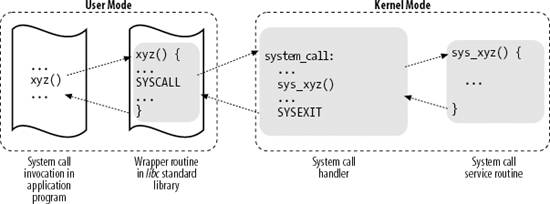
\includegraphics[width=0.8\textwidth]{imagenes/syscall.png}
	\caption{syscall}
	\end{center}
\end{figure}
~\\

\subsection{Threads}

Los threads son una especie de "mini roceso" o "proceso ligero" dentro de un proceso clásico. Los threads posibilitan el concepto de procesos secuenciales que realizan llamadas al sistema con bloqueo y de todas formas logran paralelismo.

Una manera de ver a un proceso es como si fuera una forma de agrupar recursos relacionados, como archivos abiertos, procesos hijos, etc., además de su espacio de direcciones. El otro concepto que tiene un proceso es el de hilo de ejecución, el cual tiene un contador de programa, registros con sus variables actuales y una pila. Aunque un hilo se deba ejecutar en cierto proceso, el hilo y su proceso son conceptos distintos y pueden tratarse por separado.

Lo que agregan los hilos al modelo de procesos es permitir que se lleven a cabo varias ejecuciones en el mismo entorno del proceso, que son en gram parte independientes, por lo tanto, los hilos dentro de un proceso comparten el mismo espacio de direcciones. No hay protección entre los hilos debido a que (1) es imposible y (2) no debe ser necesario. A diferencia de tener procesos diferentes, que pueden ser de distintos usuarios y hostiles entre sí, un proceso siempre es propiedad de un solo usuario, quien se supone ha creado varios hilos para que cooperen. Además de compartir un espacio de direcciones, todos los threads pueden compartir el mismo conjunto de archivos abiertos, procesos hijos, señales, etc. Al igual que un proceso tradicional, un thread puede estar en uno de varios estados: ene ejecución, bloqueado, listo o terminado.

Hay 2 formas principales de implementar una librería de threads: en espacio de usuario o en el kernel, aunque también es posible una implementación híbrida.

\subsubsection{Implementación de threads en espacio de usuario}

En este caso la librería de threads reside completamente en espacio de usuario, y el kernel no sabe nada de ellos. En lo que al kernel concierne, está administrando procesos ordinarios con un solo thread.

En este caso, cada proceso tiene su propia tabla de threads. Algunas ventajas son que cuando un thread se bloquea y se debe conmutar con otro, el procedimiento es mucho más rápido que hacer el trap al kernel. Otra ventaja es que cada proceso puede tener su propio algoritmo de planificación personalizado.

A pesar de su buen rendimiento, los threads a nivel de usuario tienen algunos problemas importantes. El primero de todos es la manera en que se implementan las llamadas al sistema de bloqueo. Si, por ejemplo, un thread lee del teclado antes de que se haya oprimido una sola tecla, es inaceptable permitir que el thread se bloquée, ya que esto también bloqueará a todos los threads del proceso. Si un thread produce un fallo de página, el kernel naturalmente bloquea a todo el proceso, llevando al mismo problema que en el caso anterior.

Otro problema es que si un thread comienza a ejecutarse, ningún otro thread en ese proceso se ejecutará a menos que el primero renuncie de manera voluntaria a la CPU, ya que dentro de un proceso no hay interrupciones.

\subsubsection{Implementación de threads en el kernel}

En este caso, en vez de tener una tabla de threads por proceso, el kernel tiene una tabla de threads que lleva la cuenta de todos los threads del sistema. Además, el kernel mantiene la tabla de procesos tradicional. Cuando un proceso desea crear un nuevo thread, realiza una llamada al kernel. Los threads del kernel no requieren de nuevas llamadas al sistema no bloqueantes, y si se produce un fallo de página, el kernel puede comprobar con facilidad si el proceso tiene otros threads que puedan ejecutarse y los ejecuta. Su principal desventaja es que el costo de una llamada al sistema es considerable. Sin embargo, hay algunos problemas que no resuelven, como qué hacer luego de un fork, o qué hilo debe hacerse cargo de una señal enviada al proceso.

\subsubsection{Implementaciones híbridas}

Una manera de combinar los métodos anteriores es utilizar threads de nivel kernel y después multiplexar los threads de nivel usuario con alguno o todos los threads de nivel kernel. El programador puede determinar cuántos hilos de kernel va a utilizar y cuántos threads de nivel usuario va a multiplexar en cada uno.


\subsection{Sincronización entre procesos}

Los bugs que surgen cuando dos o más procesos están leyendo o escribiendo en algún buffer compartido y el resultado final depende de quién se ejecuta y exactamente cuándo lo hace, se conocen como \textbf{condiciones de carrera.}

Para evitar esto, se necesita \textbf{exclusión mutua}, es decir, cierta forma de asegurar que si un proceso está utilizando una variable o archivo compartido, los demás procesos se excluirán de hacer lo mismo. La parte del programa en la que se accede a la memoria compartida se conoce como \textbf{región crítica.}

Para solucionar esto, se busca cumplir las siguientes cuatro condiciones:

\begin{itemize}
\item No puede haber dos procesos de manera simultánea dentro de sus regiones críticas.
\item No pueden hacerse suposiciones acerca de las velocidades o el número de CPUs.
\item Ningún proceso que se ejecute fuera de su región crítica puede bloquear otros procesos.
\item Ningún proceso tiene que esperar para siempre para entrar a su región crítica.
\end{itemize}

Algunas proposiciones para lograr exclusión mutua son las siguientes:

\begin{itemize}
\item \textbf{\underline{Deshabilitar interrupciones:}} en un sistema con un solo procesador, la solución más simple es hacer que cada proceso deshabilite todas las interrupciones justo después de entrar a su región crítica y las rehabilite justo después de salir. A pesar de que esto soluciona el problema de las condiciones de carrera, introduce un nuevo problema, ya que si el proceso no rehabilita las interrupciones, el sistema no podría continuar ejecutándose.

En un procesador multinúcleo, al deshabilitar las interrupciones de una CPU no se evita que las demás CPUs interfieran con las operaciones que la primera CPU está realizando. En consecuencia, se requieren esquemas más sofisticados.

\item \textbf{\underline{Variables candado:}} es una solución por software que consiste en tener una variable compartida que está en 0 cuando no hay ningún proceso en su región crítica y 1 cuando si lo hay. Este método tiene el mismo problema que el anterior, ya que si 2 procesos leen el 0 a la vez, ambos fijarán el candado en 1 y entrarán en su región crítica.

\item \textbf{\underline{Alternancia estricta:}}
~\\
\begin{figure}[h]
	\begin{center}
	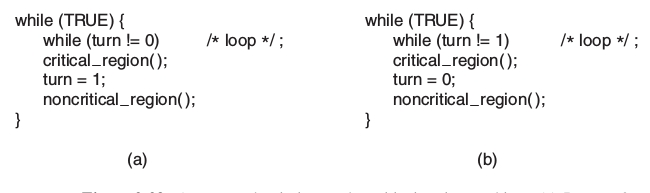
\includegraphics[width=0.8\textwidth]{imagenes/alternancia-estricta.jpg}
	\end{center}
\end{figure}
~\\

Cuando un proceso está evaluando continuamente una variable (como \textit{turn}), se dice que está haciendo \textbf{busy waiting}.

El problema con este enfoque es que si uno de los procesos es mucho más lento que el otro, este otro proceso quedará haciendo busy waiting hasta que el proceso más lento vuelva a cambiar la variable candado. Esta situación viola la condición 3 antes establecida: un proceso está siendo bloqueado por otro proceso que no está en su región crítica. Por más que evite las condiciones de carrera, no es un candidato serio como solución.
~\\

\item \textbf{\underline{Solución de Peterson:}}

\begin{figure}[h]
	\begin{center}
	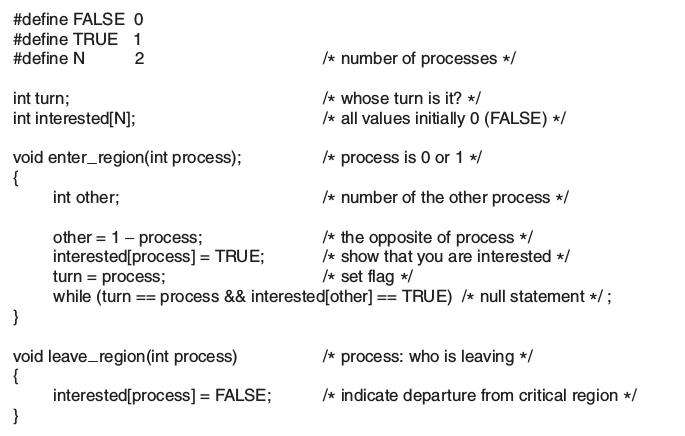
\includegraphics[width=0.8\textwidth]{imagenes/peterson.jpg}
	\end{center}
\end{figure}

\item \textbf{\underline{Instrucción TSL:}} TSL (test-and-set-lock) es una instrucción del hardware que funciona de la siguiente manera: lee el contenido de una palabra de memoria (candado) y lo guarda en un registro, y después almacena un valor distinto de cero en la dirección de memoria del candado. Se garantiza que las operaciones de leer la palabra y almacenar un valor en ella serán indivisibles; la CPU que ejecuta la instrucción TSL bloquea el bus de memoria para impedir que otras CPUs accedan a la memoria hasta que termine. Para lograr esto, se deshabilita el bus de memoria para el resto de los procesadores. Para usar la instrucción TSL necesitamos una variable compartida (candado) que coordine el acceso a la memoria compartida. Cuando candado es 0, cualquier proceso lo puede fijar en 1 mediante el uso de la instrucción TSL y después una lectura o escritura en la memoria compartida. Cuando termina, el proceso establece candado en 0 mediante una instrucción move ordinaria.

\item \textbf{\underline{sleep y wakeup:}} tanto la solución de Peterson como la solución mediante TSL son correctas, pero todas tienen el defecto de requerir busy waiting. Esto no solo desperdicia tiempo de CPU, sino que también puede tener efectos inesperados, por ejemplo, si hay 2 procesos H y L con prioridad alta y baja respectivamente, y H se ejecuta cada vez que se encuentra en el estado listo. En cierto momento, con L en su región crítica, H cambia al estado listo para ejecutarse y empieza a hacer busy waiting, pero como L nunca se planifica mientras H está en ejecución, L no puede salir de su región crítica y H queda iterando indefinidamente. A esta situación se la conoce como el problema de \textbf{inversión de prioridades}.

Una alternativa es usar ciertas primitivas para bloquear a los procesos que no pueden entrar a sus regiones críticas. Una de las más simples es el par \textbf{sleep} y \textbf{wakeup}. Como ejemplo de la forma en que se pueden usar, consideremos el problema del \textbf{productor-consumidor}: dos procesos comparten un buffer común de tamaño fijo. Uno de ellos (el productor) coloca datos en el buffer y el otro (el consumidor) los saca (esto se puede generalizar al caso de $m$ productores y $n$ consumidores).

El problema surge cuando el productor desea colocar un nuevo elemento en el buffer, pero este ya se encuentra lleno. La solución es que el productor se vaya a dormir y que se despierte cuando el consumidor haya quitado uno o más elementos, y de manera similar el consumidor se duerme si el buffer se encuentra vacío. Para llevar la cuenta del número de elementos en el buffer, necesitamos una variable (cuenta). Este método sin embargo produce condiciones de carrera, debido a que el acceso a cuenta no está restringido. Es posible que ocurra la siguiente situación: el buffer está vacío y el consumidor acaba de leer cuenta para ver si es $0$. En ese instante, el scheduler detiene al consumidor y empieza a ejecutarse el productor, el cual inserta un elemento en el buffer e incrementa cuenta, que ahora es $1$. Razonando que cuenta era antes $0$, y que por ende el consumidor debe estar dormido, el productor llama a wakeup para despertar al consumidor.

Como el consumidor todavía no estaba dormido, la señal se pierde. Cuando se vuelve a ejecutar el consumidor, evalúa el valor de cuenta que leyó antes, ve que es $0$ y pasa a dormirse. En algún momento el productor llena el buffer y se duerme. Ambos quedan dormidos para siempre.

El problema es que se envía una señal que se pierde. Una solución rápida es agregar un bit de espera, aunque esto también deja de funcionar con 3 o más procesos.

\item \textbf{\underline{Semáforos:}} un semáforo es una variable entera para contar el número de señales de despertar, almacenadas para un uso futuro. Cuenta con las funciones \textbf{down} y \textbf{up} (generalizaciones de sleep y wakeup). La función down comprueba si el valor es mayor que $0$. De ser así, disminuye el valor y sólo continúa. Si el valor es $0$, el proceso se pone a dormir sin completar la operación down por el momento. Las acciones de comprobar el valor, modificarlo y posiblemente pasar a dormir, se realizan como una sola acción atómica indivisible. Esta atomicidad es esencial para resolver problemas de sincronización y evitar condiciones de carrera.

La operación \textbf{up} incrementa el valor del semáforo. Si uno o más procesos estaban inactivos en ese semáforo, el sistema selecciona uno de ellos al \textbf{azar} y permite que complete su operación down. Por lo tanto, después de un up en un semáforo que contenga procesos dormidos, el semáforo seguirá en $0$ pero habrá un proceso dormido menos en él. La operación up también es indivisible.

En el caso del productor-consumidor, se utilizan 2 tipos de semáforos: uno es el \textbf{mutex}, que se utiliza para la exclusión mutua. Está diseñado para que un solo proceso pueda leer o escribir el buffer y sus variables asociadas en un momento dado.

El otro uso de los semáforos es para la sincronización, por ejemplo, para que el productor deje de ejecutarse cuando el buffer esté lleno, y que el consumidor deje de ejecutarse cuando esté vacío.


\item \textbf{\underline{Monitores:}} un monitor es una colección de procedimientos, variables y estructuras de datos que se agrupan en un tipo especial de módulo o paquete. Tienen una importante propiedad que los hace útiles para lograr la exclusión mutua: sólo puede haber un proceso activo en un monitor en un instante dado. Los monitores son una construcción del lenguaje de programación, por lo que el compilador sabe que son especiales y puede manejar las llamadas a las funciones del monitor en forma distinta a las llamadas a otras funciones. Es responsabilidad del compilador implementar la exclusión mutua en las entradas del monitor.

Aunque los monitores proporcionan una manera fácil de lograr la exclusión mutua, se necesita también una forma en la que los procesos se bloqueen cuando no puedan continuar. La solución está en la introducción de las \textbf{variables de condición}, junto con 2 operaciones asociadas: \textbf{wait} y \textbf{signal}. Cuando un procedimiento de monitor no puede continuar, realiza un wait en alguna variable de condición, lo cual hace que el proceso se bloquee. Un proceso, por ejemplo, el consumidor, puede despertar a su socio dormido mediante un signal en la variable de condición. Para evitar tener 2 procesos activos en el monitor al mismo tiempo, necesitamos una regla que indique lo que ocurre después de una operación signal. Hoare propuso dejar que el proceso recién despertado se ejecutara, suspendiendo el otro. Hansen propuso requerir que un proceso que realice una operación signal deba salir del monitor de inmediato.
\end{itemize}

\newpage


\section{Scheduling}

En un sistema con multiprogramación, con frecuencia se tienen varios procesos o hilos que comparten la CPU al mismo tiempo. Si solo hay una CPU disponible, hay que decidir cuál proceso se va a ejecutar a continuación. La parte del sistema operativo que realiza esa decisión se llama \textbf{scheduler} y el algoritmo que utiliza se conoce como \textbf{algoritmo de planificación}.

Casi todos los procesos alternan ráfagas de cálculos con peticiones de E/S (de disco). Por lo general la CPU opera durante cierto tiempo sin detenerse, y después se realiza una llamada al sistema para leer o escribir datos en un archivo. Cuando se completa la llamada al sistema, la CPU realiza cálculos de nuevo y así sucesivamente. A los procesos que invierten la mayor parte de su tiempo realizando cálculos se los llama limitados a cálculos, mientras que a los que están la mayor parte del tiempo esperando la E/S se los llama limitados a E/S (I/O-bound). A medida que las CPUs se vuelven más rápidas, los procesos tienden a ser más limitados a E/S, por lo tanto estos procesos deben obtener rápidamente la oportunidad de ejecutarse para emitir su petición de disco y mantenerlo ocupado.

Los algoritmos de planificación se pueden dividir en dos categorías según cómo manejan las interrupciones de reloj: un algoritmo \textbf{no apropiativo} (nonpreemptive) selecciona un proceso para ejecutarlo y después sólo deja que se ejecute hasta que el mismo se bloquea o hasta que libere la CPU en forma voluntaria. No se toman decisiones de planificación durante las interrupciones de reloj. Una vez que se haya completado el procesamiento de la interrupción de reloj, se reanuda la ejecución del proceso que estaba antes de la interrupción, a menos que un proceso de mayor prioridad esté listo para correr.

Por el contrario, un algoritmo de planificación \textbf{apropiativo} (preemptive) selecciona un proceso y deja que se ejecute por un máximo de tiempo fijo. Si sigue en ejecución al final del intervalo de tiempo, se suspende y el scheduler selecciona otro proceso para ejecutarlo. Para llevar a cabo la planificación apropiativa, es necesario que ocurra una interrupción de reloj al final del intervalo para que la CPU regrese el control al scheduler.

\subsection{Categorías de los algoritmos de planificación}

\begin{itemize}

\item \textbf{\underline{Procesamiento por lotes:}} en los sistemas de procesamiento por lotes no hay usuarios que esperen una respuesta rápida a una petición corta. En consecuencia, son aceptables los algoritmos no apropiativos, ya que reducen la conmutación de procesos y por ende mejora el rendimiento.

\item \textbf{\underline{Interactivos:}} en este caso la apropiación es esencial para evitar que un proceso acapare la CPU y niegue el servicio a los demás.

\item \textbf{\underline{De tiempo real:}} en los sistemas de tiempo real, aunque parezca extraño, la apropiación a veces no es necesaria debido a que los procesos saben que no se pueden ejecutar durante períodos extensos. La diferencia con los sistemas interactivos es que los sistemas de tiempo real sólo ejecutan programas destinados para ampliar la aplicación en cuestión.

\end{itemize}

Algunas metas de los algoritmos de planificación que aplican a todos los sistemas son:

\begin{itemize}
\item Equidad: otorgar a cada proceso una parte justa de la CPU.
\item Aplicación de políticas: verificar que se lleven a cabo las políticas establecidas.
\item Balance: mantener ocupadas todas las partes del sistema.
\end{itemize}

En los sistemas de procesamiento por lotes se utilizan tres métricas para verificar el desempeño de los sistemas: rendimiento, tiempo de retorno y utilización de la CPU. El \textbf{rendimiento (throughput)} es el número de trabajos por hora que completa el sistema. El \textbf{tiempo de retorno} es el tiempo estadísticamente promedio desde el momento en que se envía un trabajo por lotes, hasta el momento en que se completa. Es el tiempo de respuesta que tiene el usuario.

Un algoritmo que maximiza el rendimiento no necesariamente minimiza el tiempo de retorno. Por ejemplo, dada una mezcla de trabajos cortos y largos, un scheduler que siempre ha ejecutado trabajos cortos y nunca uno largo puede tener un rendimiento excelente pero a expensas de un terrible tiempo de retorno para trabajos largos.

Para los sistemas interactivos se aplican distintas métricas. La más importante es minimizar el \textbf{tiempo de respuesta}, es decir, el tiempo que transcurre entre emitir un comando y obtener el resultado.

Los sistemas de tiempo real tienen diferentes metas de planificación. Se caracterizan por tener tiempos límite que deben cumplir. Por ejemplo, si una computadora está controlando un dispositivo que produce datos a un paso regular, al no ejecutar el proceso de recolección de datos a tiempo se podría perder información.

\subsection{Planificación en sistemas de procesamiento por lotes}

\subsubsection{First-Come, First-Served (FCFS)}

Con este algoritmo, la CPU se asigna a los procesos en el orden en el que la solicitan. Es un algoritmo no apropiativo, por lo tanto los procesos no se interrumpen por haberse ejecutado demasiado tiempo. Si el proceso en ejecución se bloquea, el primer proceso en la cola se ejecuta a continuación. Cuando un proceso bloqueado pasa al estado listo, al igual que un trabajo recién llegado, se coloca al final de la cola. Tiene como ventaja que es sencillo de implementar.

\subsubsection{Shortest Job First (SJF)}

Es un algoritmo de procesamiento por lotes no apropiativo, que asume que los tiempos de ejecución se conocen de antemano. Está orientado a maximizar el throughput. Sólo es óptimo cuando todos los trabajos están disponibles al mismo tiempo.

\subsubsection{Shortest Remaining Time Next (SRTN)}

Es una versión apropiativa de SJF.


\subsection{Planificación en sistemas interactivos}

\subsubsection{Round Robin}

A cada proceso se le asigna un intervalo de tiempo, conocido como \textbf{quantum}, durante el cual se le permite ejecutarse. Si el proceso se sigue ejecutando al final del quantum, la CPU es apropiada para dársela a otro proceso. Si el proceso se bloquea o termina antes de que haya transcurrido el quantum, la conmutación se realiza en ese momento.

La única cuestión interesante relacionada con este algoritmo es la longitud del quantum. Si se establece un quantum demasiado corto se producen demasiadas conmutaciones de procesos y se reduce la eficiencia de la CPU, pero si es demasiado largo se puede producir una mala respuesta a las peticiones interactivas cortas.

\subsubsection{Planificación por prioridad}

Round Robin hace la suposición implícita de que todos los procesos tienen igual importancia. La idea básica es: a cada proceso se le asigna una prioridad y el proceso ejecutable con la prioridad más alta es el que se puede ejecutar.

Para evitar que los procesos con alta prioridad se ejecuten de manera indefinida, el scheduler puede reducir la prioridad del proceso actual en cada pulso del reloj. De manera alternativa, a cada proceso se le puede asignar un quantum de tiempo máximo que tiene permitido ejecutarse.

Las prioridades se pueden asignar de manera estática o dinámica. Un ejemplo de esto último sería cuando algunos procesos que están muy limitados por la E/S requieren la CPU. En ese caso, el proceso debe recibir la CPU de inmediato para dejar que inicie su siguiente petición de E/S.

\subsubsection{Múltiples colas}

Se utilizan varias colas que representan distintas clases de prioridas. Por ejemplo, los procesos en la clase más alta se ejecutan durante un quantum, los de la siguiente clase durante 2 quantums, etc. Cada vez que un proceso utiliza todos los quantums que tenía asignados, se mueve una clase hacia abajo en la jerarquía.

\newpage

\section{Administración de memoria}

La parte del sistema operativo que administra (parte de) la jerarquía de memoria se conoce como \textbf{administrador de memoria}. Su trabajo es administrar la memoria con eficiencia: llevar el registro de cuáles partes de la memoria están en uso, asignar memoria a los procesos cuando la necesiten y desasignarla cuando terminen.

\subsection{Sin abstracción de memoria}

La abstracción más simple de memoria es ninguna abstracción. Cada programa ve simplemente la memoria física. Aunque pueden haber varios procesos en memoria corriendo a la vez, pueden ocurrir errores tales como que un proceso pise la memoria de otro, o que un proceso, a la hora de hacer un JMP, salte a una posición incorrecta por haber hecho referencia a una posición absoluta.

\subsection{Espacios de direcciones}

Hay que resolver dos problemas para permitir que haya varias aplicaciones en memoria al mismo tiempo sin que interfieran entre sí: protección y reubicación. Una solución es inventar una nueva abstracción para la memoria: el espacio de direcciones. Un espacio de direcciones crea un tipo de memoria abstracta, es el conjunto de direcciones que puede utilizar un proceso para direccionar memoria.

El uso de registros base y límite es una manera fácil de proporcionar a cada proceso su propio espacio de direcciones privado. Una desventaja de este método es la necesidad de realizar una suma y una comparación en cada referencia a memoria.

\subsection{Administración de memoria libre}

Hay 2 formas de llevar el registro del uso de la memoria: mapas de bits y listas libres.

\begin{itemize}

\item \textbf{\underline{Mapas de bits:}} en este esquema, la memoria se divide en unidades de asignación, que pueden ser unas cuantas palabras o varios kilobytes. Para cada unidad de asignación hay un bit correspondiente en el mapa de bits. El problema principal es que, cuando se quiere cargar un proceso de k unidades a la memoria, se debe buscar en el mapa una serie de k bits consecutivos con el valor 0, lo cual es una operación lenta.

\item \textbf{\underline{Listas libres:}} se mantiene una lista ligada de segmentos de memoria asignados y libres, en donde un segmento contiene un proceso o es un hueco vacío entre 2 procesos.

Cuando los procesos y huecos se mantienen en una lista ordenada por dirección, se pueden utilizar varios algoritmos para asignar memoria a un proceso creado.

El algoritmo más simple es el \textbf{First-Fit}: se reserva el primer bloque que sea lo suficientemente grande.

Otro algoritmo es el \textbf{Best-Fit}: reserva el bloque más pequeño entre todos los bloques que sean lo suficientemente grandes. Hay que recorrer toda la lista. Sorprendentemente, provoca más desperdicio de memoria que First-Fit, ya que tiende a llenar la memoria con huecos pequeños e inutilizables.

Para resolver el problema de dividir las coincidencias casi exactas en un proceso y en un pequeño hueco, se puede utilizar el algoritmo \textbf{Worst-Fit}, el cual reserva el bloque más grande disponible. Tampoco es muy buena idea.

Otro algoritmo de asignación es el \textbf{Quick-Fit}, el cual mantiene listas separadas para algunos de los tamaños más comunes solicitados. Tiene la misma desventaja que todos los esquemas que se ordenan por el tamaño del hueco: cuando un proceso termina o es intercambiado, buscar en sus vecinos para ver si es posible una fusión es un proceso costoso. Todos estos algoritmos sufren de \textbf{fragmentación externa}. La fragmentación externa se da cuando existe suficiente memoria para satisfacer un pedido, pero esta no es contigua. Una solución al problema de la fragmentación externa es la compactación. Otra solución es la paginación. La paginación permite que el espacio de direcciones físicas de un proceso no sea necesariamente continuo. Con paginación no hay fragmentación externa, ya que cualquier frame puede ser reservado para un proceso. Sin embargo, puede haber \textbf{fragmentación interna}, ya que los frames son de tamaño fijo, y puede que los requerimientos de memoria no coincidan con los del tamaño del frame. Por lo tanto, el último frame reservado no será utilizado del todo. En el peor caso se desperdician 4KB - 1B = 4095B.

\end{itemize}


\subsection{Memoria Virtual}

La idea básica es que cada programa tiene su propio espacio de direcciones, el cual se divide en trozos llamados \textbf{páginas}. Cada página es un rango contiguo de direcciones, las cuales se asocian a la memoria física, pero no todas tienen que estar en memoria para poder ejecutar el programa. Cuando el programa hace referencia a una parte de su espacio de direcciones que no está en la memoria física, el sistema operativo recibe una alerta para buscar la parte faltante y volver a ejecutar la instrucción que falló. En cierto sentido, la memoria virtual es una generalización de la idea de los registros base y límite.

\subsection{Paginación}

Las direcciones de memoria generadas por un programa se conocen como \textbf{direcciones virtuales}. En las computadoras sin memoria virtual, la dirección física se coloca directamente en el bus de memoria. Cuando se utiliza memoria virtual, las direcciones virtuales no van al bus de memoria, sino a la \textbf{MMU} (Memory Management Unit), que asocia las direcciones virtuales a las físicas.

El espacio de direcciones virtuales se divide en unidades de tamaño fijo llamadas \textbf{páginas}. Las unidades correspondientes en la memoria física se llaman \textbf{marcos de página}. Las páginas y los marcos de página suelen ser del mismo tamaño, y suelen ser de 4 KB. Las transferencias entre la RAM y el disco siempre son de páginas completas. Si el programa hace referencia a una página que no está presente, la CPU hace un trap al sistema operativo. A este trap se lo llama \textbf{page fault}.

Los tamaños de página son potencia de 2 ya que dentro de la MMU se utilizan parte de los bits de la dirección virtual para seleccionar una página, y los restantes bits para indexar dentro de esa página. El número de página se utiliza como índice en la \textbf{page table.}

\subsection{Page Tables}

En una implementación simple, el mapeo de direcciones virtuales a físicas se realiza de la siguiente manera: la dirección virtual se divide en un número de página virtual (bits de mayor orden) y en un desplazamiento (bits de menor orden).

En cualquier sistema de paginación hay que abordar dos cuestiones principales:

\begin{itemize}
\item La asociación entre una dirección virtual y una física debe ser rápida.

\item Si el espacio de direcciones virtuales es grande, la page table será grande.
\end{itemize}

El primer punto es una consecuencia del hecho de que la asociación virtual a física debe realizarse en cada referencia a memoria.

El segundo punto se deriva del hecho de que todas las computadoras modernas utilizan direcciones virtuales de 32 o 64 bits. Con un tamaño de página de 4 KB y un espacio de direcciones de 32 bits, habrá 1 millón de páginas, y por lo tanto la page table tendrá 1 millón de entradas.

La solución para acelerar el mapeo de direcciones virtuales a físicas fue equipar a las computadoras con una cache especial que guarde las asociaciones entre direcciones virtuales y físicas sin pasar por la page table. Esta cache se llama \textbf{TLB} (Translation Lookaside Buffer). La TLB funciona de la siguiente manera: cuando se presenta una dirección virtual a la MMU, ésta chequea en paralelo si el número de página virtual está presente en la TLB, es decir, chequea todas las entradas en forma simultánea. Si se encuentra una coincidencia válida y el acceso no viola los bits de protección, el page frame se toma directamente sin pasar por la tabla de páginas. En caso contrario, se realiza una búsqueda ordinaria en la tabla de páginas, se desaloja una entrada de la TLB y se la reemplaza con la entrada que se acaba de buscar.

Hasta ahora supusimos que toda máquina con memoria virtual paginada tiene page tables reconocidas por el hardware, más un TLB. En este diseño, la administración y el manejo de fallas del TLB se realiza por completo mediante el hardware de la MMU. Sin embargo, esta suposición ya no es correcta, ya que en muchas máquinas modernas se hace casi toda la administración de páginas mediante software. En estas máquinas, las entradas del TLB se cargan de manera explícita mediante el sistema operativo. Cuando no se encuentra una coincidencia en el TLB, en vez de que la MMU vaya a las tablas de páginas para buscar y obtener la referencia a la página que se necesita, solo genera un fallo del TLB y pasa el problema al sistema operativo. El sistema debe buscar la página, eliminar una entrada del TLB, introducir la nueva página y reiniciar la instrucción que originó el fallo.

El otro problema que había era el de espacios de direcciones virtuales muy extensos. Algunas maneras de lidiar con esto son las tablas de páginas multinivel.


\subsection{Tablas de páginas multinivel}

La idea de este método es evitar mantener todas las tablas de páginas en memoria, en especial aquellas que no se necesitan. Para lograr esto, se divide la tabla de páginas en partes más pequeñas. Una manera es usar paginación de 2 niveles, en donde la tabla de páginas también es paginada. En el caso de una máquina de 32 bits con un tamaño de página de 4 KB, las direcciones de memoria se dividen en:

~\\

\begin{figure}[h]
	\begin{center}
	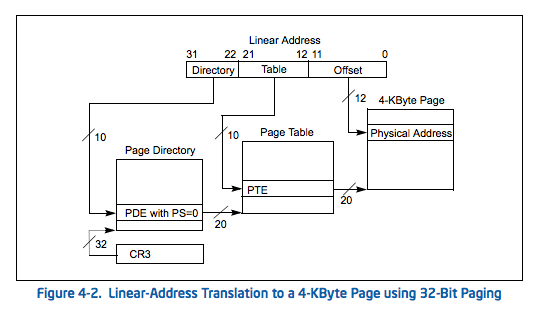
\includegraphics[width=0.8\textwidth]{imagenes/32-bit-4k-paging.png}
	\end{center}
\end{figure}

~\\

Todos los procesos activos deben tener un Page Directory asignado; sin embargo, no es necesario reservar memoria para todas las tablas de páginas del proceso, sino solo para las que necesita. Con el esquema de paginación simple de 1 nivel, la Page Table de cada proceso tendría $2^{20}$ entradas, y con 4 bytes por entrada, serían 4 MB por proceso. El esquema de 2 niveles reduce la cantidad de memoria requerida haciendo que sólo se usen tablas de páginas para aquellas regiones de memoria virtual realmente utilizadas por el proceso.

\subsection{Algoritmos de reemplazo de páginas}

Cuando ocurre un fallo de página, el sistema operativo tiene que elegir una página para desalojarla de memoria y hacer espacio para la página entrante. Algunos algoritmos de reemplazo de páginas son:


\begin{itemize}
\item \textbf{\underline{First In First Out (FIFO):}} el sistema operativo mantiene una lista de todas las páginas actualmente en memoria. En un fallo de página, se elimina la página que está en la parte frontal y la nueva página se agrega al final de la lista.

\item \textbf{\underline{Reloj:}} en este caso, los marcos de página se mantienen en una lista circular, con un puntero a la página más antigua. Cuando ocurre un fallo de página, la página apuntada se inspecciona. Si el bit R es $0$ la página se desaloja, se inserta la nueva página en su lugar y el puntero se avanza una posición. Si R es $1$, se borra y el puntero avanza. Esto se repite hasta encontrar una página con R = $0$.

\item \textbf{\underline{Least Recently Used (LRU):}} cuando ocurre un fallo de página, se descarta la página que no se haya utilizado durante la mayor longitud de tiempo. Aunque es realizable, no es barato.

Una posible implementación de este algoritmo mediante hardware es la siguiente: para una máquina con $n$ marcos de página, se mantiene una matriz de $nxn$ bits (inicialmente todos en $0$). Cada vez que se hace referencia a la página k, el hardware establece todos los bits de la fila k en $1$ y después todos los bits de la columna k en $0$. En cualquier instante, la fila cuyo valor binario sea menor es la de uso menos reciente.

\item \textbf{\underline{Not Frequently Used (NFU):}} este algoritmo requiere un contador de software asociado con cada página, que al principio es $0$. En cada interrupción de reloj, se agarra cada una de las páginas en memoria y se agrega el bit R, que es $0$ o $1$, al contador. Los contadores llevan la cuenta aproximada de la frecuencia con que se hace referencia a cada página. Cuando ocurre un page fault, se sustituye la página que tenga el menor contador.
\end{itemize}


\subsection{Page Fault}

Cuando ocurre un page fault, se ejecutan los siguientes pasos:

\begin{itemize}
\item Se emite un page fault, que es una excepción. La atrapa el kernel.
\item Se guardan el IP y otros registros en la pila.
\item El kernel determina que la excepción es de tipo page fault y llama al handler de la interrupción.
\item Se chequea que la dirección virtual que se estaba buscando sea válida y que el proceso que la pide tenga permisos para accederla. Si no es así, se mata al proceso.
\item Se selecciona un page frame libre si lo hubiese, y sino se libera uno mediante el algoritmo de reemplazo de páginas.
\item Si la página tenía el bit dirty prendido, hay que bajarla a disco. Es decir, el proceso del kernel que maneja E/S debe ser suspendido, generándose un cambio de contexto y permitiendo que otros ejecuten. La página se marca como busy para evitar que se use.
\item Cuando el SO es notificado de que se terminó de bajar la página a disco, comienza otra operación de E/S, esta vez para cargar la página que hay que subir.
\item Cuando llega la interrupción que indica que la E/S para subir la página terminó, hay que actualizar la tabla de páginas para indicar que está cargada.
\item La instrucción que causó el page fault se recomienza, tomando el IP que había quedado en el stack y los valores anteriores de los registros.
\item Se devuelve el control al proceso de usuario. En algún momento, el scheduler lo va a hacer correr de nuevo, y cuando reintente la instrucción la página ya va a estar en memoria.
\end{itemize}

\newpage
\section{Deadlocks}

En un sistema con multiprogramación, distintos procesos compiten por un número finito de recursos. Un proceso pide recursos; si los recursos no están disponibles, el proceso se bloquea. Puede suceder que los procesos bloqueados nunca se despierten, porque los recursos que pidieron están siendo retenidos por otros procesos bloqueados a su vez por esperar a los recursos del primer proceso.  Esta situación se denomina \textbf{deadlock}.

Una clase principal de deadlocks involucra a los recursos, que pueden ser de hardware o de software. Los recursos son de dos tipos: \textbf{apropiativos} y \textbf{no apropiativos}. Un recurso apropiativo es uno que se puede quitar al proceso que lo posee sin efectos dañinos. Un ejemplo es la memoria. Un recurso no apropiativo es uno que no se puede quitar a su propietario sin hacer que el cómputo falle. Un ejemplo sería una grabadora de DVD. En general, los deadlocks involucran recursos no apropiativos.

\subsection{Condiciones necesarias para un deadlock}

Se deben cumplir 4 condiciones simultáneamente para que se de un deadlock:

\begin{itemize}
\item  \textbf{\underline{Exclusión Mutua:}} el recurso se asigna en un momento dado a sólo un proceso, o está disponible en caso contrario.
\item  \textbf{\underline{Hold and Wait:}} debe existir un proceso que esté reteniendo al menos un recurso y esté esperando para conseguir recursos adicionales que están siendo retenidos por otro proceso.
\item  \textbf{\underline{No Preemption:}} los recursos otorgados a un proceso no se le pueden quitar por la fuerza. Estos deben ser liberados de forma explícita por el proceso que los contiene.
\item  \textbf{\underline{Circular Wait:}} debe haber una cadena circular de 2 o más procesos, cada uno de los cuales espera un recurso retenido por el siguiente miembro de la cadena.
\end{itemize}

En general, se utilizan 4 estrategias para lidiar con los deadlocks:

\begin{enumerate}[1]
\item Ignorar el problema.
\item Detección y recuperación.
\item Evitarlos en forma dinámica mediante la asignación cuidadosa de los recursos.
\item Prevención, al evitar estructuralmente una de las 4 condiciones requeridas.
\end{enumerate}

\subsection{Detección y recuperación}

Cuando se utiliza esta técnica, el sistema no trata de evitar los deadlocks, sino que intenta detectarlos cuando ocurren y luego realiza cierta acción para recuperarse del hecho.

El caso más sencillo es cuando sólo existe un recurso de cada tipo. Para un sistema así, se puede construir un gráfico de recursos. Si contiene 1 o más ciclos, existe un deadlock. A la hora de implementarlo, existen algoritmos para detectar ciclos en grafos.

Una vez detectado el deadlock, existen varias maneras de recuperarse:

\begin{itemize}
\item  \textbf{\underline{Recuperación por medio de apropiación:}} en este caso se quita temporalmente el recurso al proceso y se lo otorga a otro. Con frecuencia es difícil o imposible recuperarse de esta manera.
\item  \textbf{\underline{Recuperación a través del retroceso:}} en este caso los procesos realizan puntos de comprobación en forma periódica. Esto significa que su estado se escribe en un archivo para poder reiniciarlo más tarde. Cuando se detecta un deadlock, un proceso que posee un recurso necesario se revierte a un punto en el tiempo antes de que haya adquirido el recurso.
\item  \textbf{\underline{Recuperación a través de la eliminación de procesos:}} se elimina a uno de los procesos en el ciclo.
\end{itemize}
\newpage


\section{Sistemas de Archivos}

Los archivos son un mecanismo de abstracción. Proporcionan una manera de almacenar información en el disco y leerla después. Esto se debe hacer de tal forma que se proteja al usuario de los detalles acerca de cómo y dónde se almacena la información, y cómo funcionan los discos en realidad.

Los sistemas de archivos se almacenan en discos, los cuales se pueden dividir en una o más particiones, con sistemas de archivos independientes en cada partición. El sector $0$ del disco se conoce como el \textbf{MBR} (Master Boot Record) y se utiliza para arrancar la computadora. El final de la MBR contiene la tabla de particiones, la cual proporciona las direcciones de inicio y fin de cada partición.

Una posible distribución del sistema de archivos sería:
\\


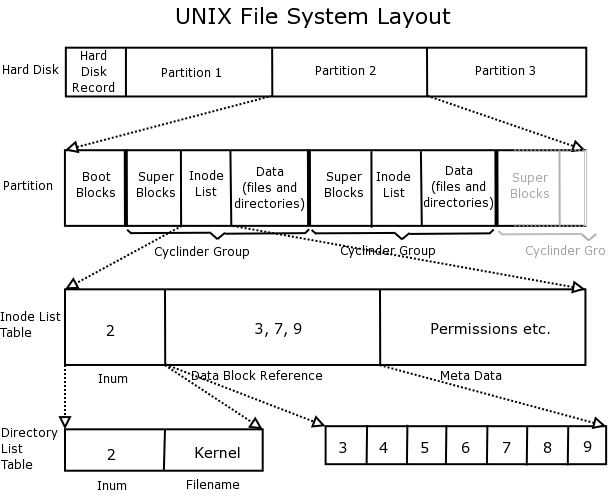
\includegraphics[scale=0.4]{imagenes/file-system.jpg}
\\


El \textbf{superbloque} contiene todos los parámetros clave acerca del sistema de archivos y se lee en la memoria cuando se entra en contacto con el sistema de archivos por primera vez.

\subsection{Implementación de archivos}

\subsubsection{Asignación continua}

El esquema de asignación continua más simple es almacenar cada archivo como una serie contigua de bloques en disco. Así, en un disco con bloques de 1 KB, a un archivo de 50 KB se le asignarían 50 bloques consecutivos. Las ventajas de este método son 2: es fácil de implementar y el rendimiento de lectura es excelente. La desventaja es que los discos se fragmentan. Este esquema, sin embargo, es útil en los CD's.

\subsubsection{Asignación de lista enlazada}

A diferencia de la asignación contigua, en este método se puede utilizar cada bloque del disco y no se pierde espacio debido a la fragmentación.

En este caso, como los bloques no son continuos, se puede tener una tabla en memoria con punteros a otras partes de la tabla, los cuales representan la cadena de bloques del archivo. La principal desventaja de este método es que toda la tabla debe estar en memoria todo el tiempo. Esta tabla en memoria principal se conoce como \textbf{FAT} (File Allocation Table).

\subsubsection{Nodos-i}

Otro método para llevar un registro de qué bloques pertenecen a cada archivo es asociar a cada archivo una estructura de datos llamada \textbf{nodo-i} (nodo-índice), la cual lista los atributos y las direcciones de disco de los bloques del archivo. Una ventaja de este método con respecto a los anteriores, es que el nodo-i necesita estar en memoria sólo cuando está abierto el archivo correspondiente.

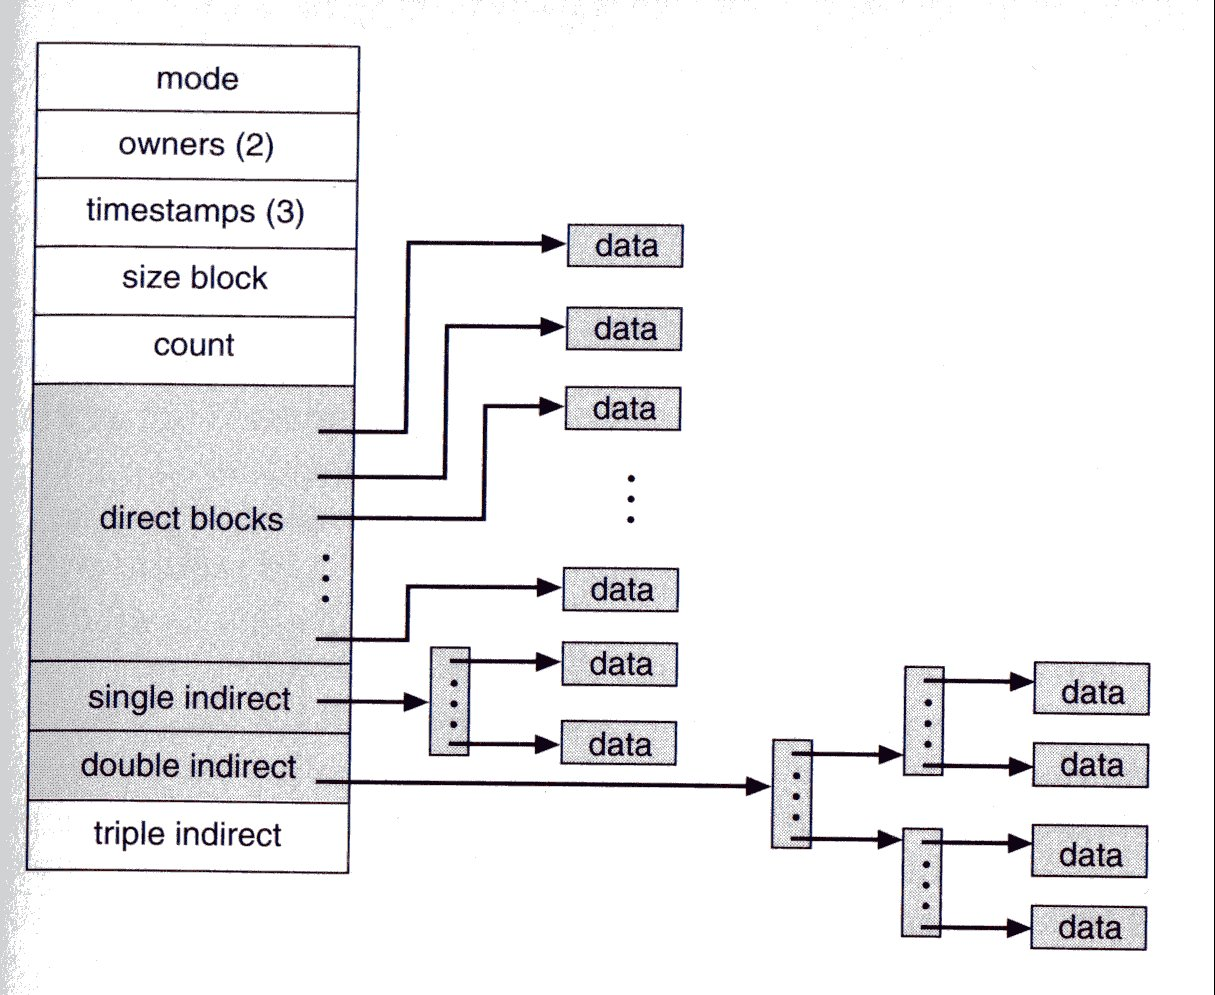
\includegraphics[scale=1]{imagenes/inode.jpg} 


\subsection{Journaling File System}

La idea de estos file systems es proveer rebustez ante las fallas, manteniendo un registro de lo que va a realizar el sistema de archivos antes de hacerlo, por lo que si el sistema falla antes de poder realizar su trabajo, al momento de re-arrancar el sistema puede buscar en el registro para ver lo que estaba ocurriendo al momento de la falla y terminar el trabajo. NTFS, Ext 3 y ReiserFS son ejemplos de JFS.

Para que funcione el sistema por bitácora, las operaciones registradas deben ser idempotentes, es decir, que pueden repetirse todas las veces que sea necesario sin peligro.

\subsection{Virtual File Systems}

Sirven para integrar múltiples sistemas de archivos en una estructura ordenada. La idea clave es abstraer la parte del sistema de archivos que es común para todos los sistemas de archivos y poner ese código en una capa separada que llame a los sistemas de archivos concretos subyacentes. Todas las llamadas al sistema relacionadas con archivos se dirigen al sistema de archivos virtual, el cual hace de interfaz para los procesos de usuario (la interfaz de POSIX). Esta es la interfaz superior.

El VFS también tiene una interfaz inferior paa los sistemas de archivos concretos.
\\


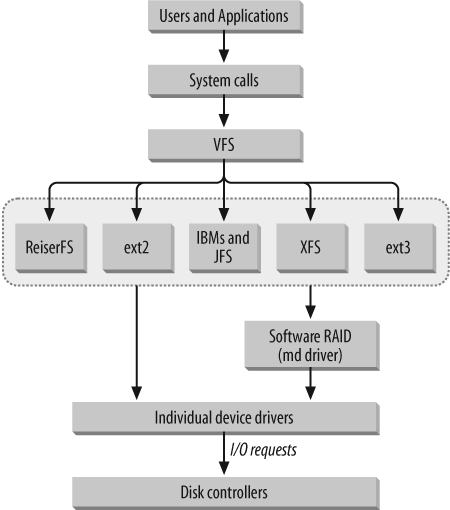
\includegraphics[scale=1]{imagenes/vfs.png}


\subsection{Administración del espacio en disco}

Hay 2 métodos utilizados para llevar el registro de los bloques libres. El primero consiste en utilizar una lista enlazada de bloques de disco, donde cada bloque contiene tantos números de bloques de disco libres como pueda.

La otra técnica es el mapa de bits. Un disco con $n$ bloques requiere un mapa de bits de $n$ bits.

\newpage

\section{Discos}

Los datos son almacenados en la superficie del plato en pistas y sectores. Las pistas son circulos concéntricos, y los sectores son divisiones de las pistas. Un sector contiene una cantidad fija de bytes. Los sectores se agrupan en clusters.

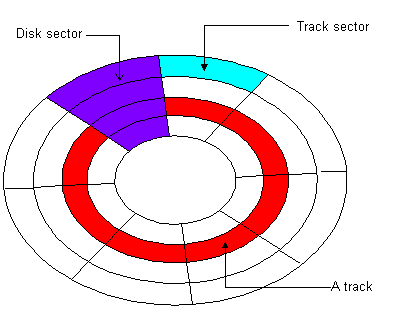
\includegraphics[scale=1]{imagenes/disco.png}


\subsection{Backup}

Tipos de backup:

\begin{itemize}
\item \underline{\textbf{Total:}} hago una copia de todo.
\item \underline{\textbf{Diferencial:}} guardo los cambios desde la última total.
\item \underline{\textbf{Incremental:}} guardo los cambios desde la última copia, sea incremental, total o diferencial.
\end{itemize}

Restaurar la información con backup:

\begin{itemize}
\item \underline{\textbf{Total:}} trivial, copio todo.
\item \underline{\textbf{Diferencial:}} obtener copia anterior y aplicar cambios
\item \underline{\textbf{Incremental:}} aplicar todas las incrementales hasta la última total o diferencial, y aplicar esa.
\end{itemize}

\subsection{RAID}

Significa Redundant Array of Inexpensive Disks. Se suelen usar "niveles", que corresponden a maneras de organizar los discos.

\subsubsection{RAID 0}

Tenemos 2 discos, ponemos un bloque de datos en cada uno (stripping).

Ventajas: todo el espacio de disco se usa para datos útiles. Mejora la performance ya que puedo hacer operaciones en paralelo.


Desventajas: cero redundancia extra. Es el doble probable que, por fallo de disco, pierda datos.

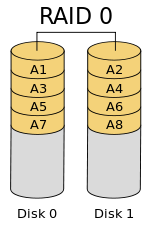
\includegraphics[scale=1]{imagenes/raid0}


\subsection{RAID 1}

Tenemos 2 discos. Duplicamos los datos.

Ventajas: redundancia. Se me tienen que caer los 2 discos para perder los datos. Las lecturas son rápidas, porque tengo dos controladoras.


Desventajas: Tengo que escribir en dos discos. Perdí un disco de almacenamiento util en redundancia.

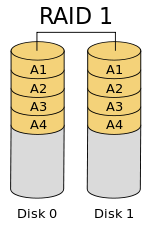
\includegraphics[scale=0.82]{imagenes/raid1}

\subsection{RAID 2}
\begin{itemize}
\item Implementa Hamming (7,4): 7 discos, 4 de datos, 3 para Hamming.
\item Leer requiere usar todas las controladoras
\item Habría que escribir demasiados discos para actualizarlo bien.
\item Strip a nivel de bit: en el primero se guardan los bits 1, 4, ...
\end{itemize}

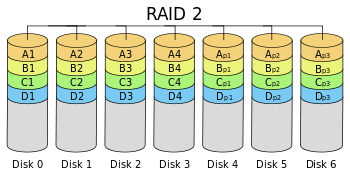
\includegraphics[scale=1]{imagenes/raid2}

\subsection{RAID 3}

\begin{itemize}
\item Strip a nivel de byte, usa paridad para corrección de errores.
\item Usa menos discos
\item Disco de paridad en todos los accesos: se gasta más rápido.
\end{itemize}

Una de las características de RAID 3 es que generalmente no puede atender múltiples pedidos simultáneamente, ya que cualquier bloque de datos va a estar repartido en todos los discos.

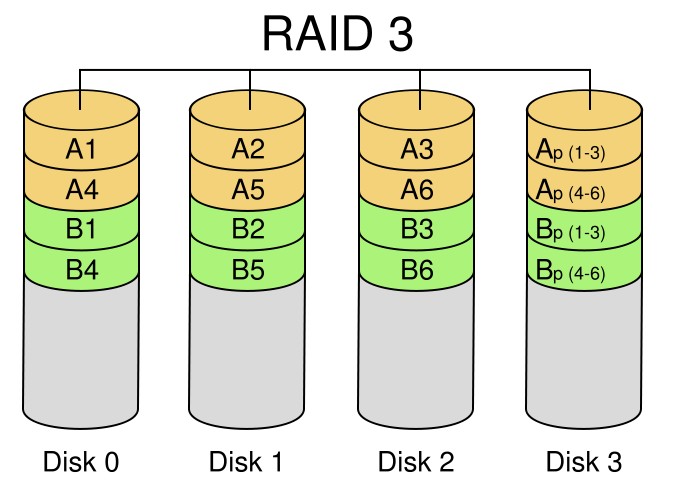
\includegraphics[scale=0.4]{imagenes/raid3}

\subsection{RAID 4}

Usa un strip a nivel de bloque, y disco único de paridad.

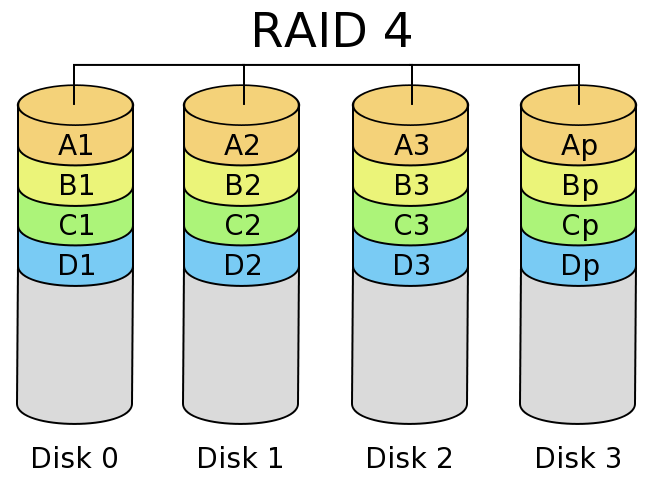
\includegraphics[scale=0.4]{imagenes/raid4}

\subsection{RAID 5}

\begin{itemize}
\item Similar al RAID 4: stripping a nivel de bloque, usa paridad.
\item Paridad distribuida mediante stripping
\item Resiste la caída de un disco usando la redundancia.
\item Requiere al menos 3 discos.
\end{itemize}

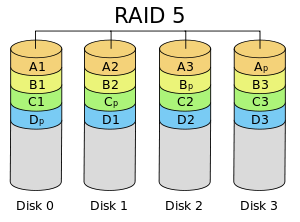
\includegraphics[scale=1]{imagenes/raid5}

\subsection{RAID 6}

\begin{itemize}
\item RAID 5 mas otro bloque de paridad.
\item Resiste la caída de hasta 2 discos.
\end{itemize}

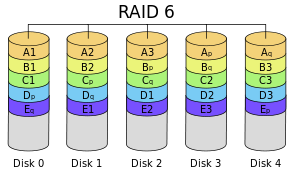
\includegraphics[scale=1]{imagenes/raid6}

\subsection{RAID 0+1}

\begin{itemize}
\item Es un mirror de stripes
\item La capacidad usable es la misma que la de RAID 1, donde la mitad de la capacidad se usa para reflejar la otra mitad.
\end{itemize}

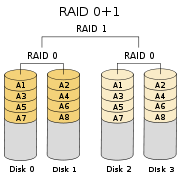
\includegraphics[scale=1.3]{imagenes/raid0+1}

\subsection{RAID 1+0}

\begin{itemize}
\item Es un stripe de mirrors
\item Requiere de mínimo 4 discos
\item Excelente redundancia y performance
\end{itemize}

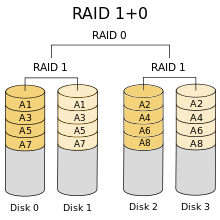
\includegraphics[scale=1.3]{imagenes/raid1+0}

En RAID 1+0, los datos están reflejados dentro de cada grupo. En RAID 0+1, los datos están reflejados a través de los distintos grupos. El RAID 0+1 tiene menos tolerancia a fallos. Si 2 discos en cada grupo fallan, por ejemplo el 1 y el 3, falla todo el sistema.

Es preferible RAID 1+0 antes que RAID 0+1.

\newpage

\section{Seguridad}

La seguridad de la información se entiende como la preservación de las siguientes características:

\begin{itemize}
\item \textbf{\underline{Confidencialidad:}} significa que los datos privados de un usuario deben permanecer privados.
\item \textbf{\underline{Integridad:}} usuarios no autorizados no deben poder modificar datos de otros usuarios sin su permiso.
\item \textbf{\underline{Disponibilidad:}} significa que nadie debería poder perturbar el funcionamiento normal del sistema.
\end{itemize}

\subsection{Permisos}

Existen distintos mecanismos para controlar el acceso a los recursos:

\begin{itemize}
\item \textbf{\underline{Dominios de protección:}} un sistema contiene varios recursos (objetos) que necesitan ser protegidos. Estos objetos pueden ser hardware (CPU, memoria, disco) o software (procesos, archivos, semáforos). Cada objeto tiene un nombre único y un conjunto finito de operaciones que los procesos tienen permitido llevar a cabo sobre ellos.

Un dominio (asociado a un sujeto) es un par (objeto, permisos). Cada par especifica un objeto y un subconjunto de las operaciones que se pueden realizar sobre dicho objeto. Un dominio se puede corresponder con un usuario particular o con un grupo de usuarios.

Se suele aplicar un principio muy común, el principio de mínimo privilegio.

En el caso particular de UNIX, el dominio de un proceso se define por su UID y su GID. Dados estos 2 valores, se puede hacer una lista de todos los objetos que pueden ser accedidos, y si pueden ser accedidos para lectura, escritura o ejecución.

Cuando un proceso ejecuta un archivo con el bit SETUID o SETGID prendido, adquiere un nuevo UID o GID, lo cual resulta en un cambio de dominio.

Este esquema se puede implementar como una matriz de protección o de control de acceso, donde para cada dominio y para cada objeto, se pueden ver los permisos que el dominio tiene sobre el objeto. También se pueden incluir los dominios a los que un dominio en particular puede entrar.

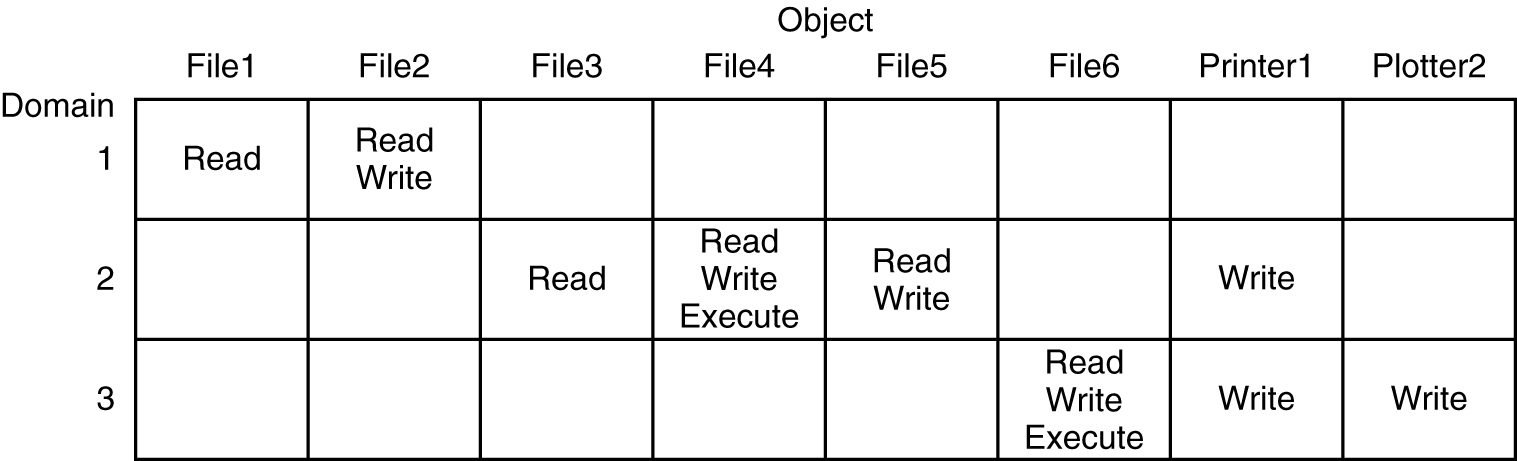
\includegraphics[scale=1]{imagenes/protection-matrix}

\item \textbf{\underline{Listas de Control de Acceso (ACL):}} como la matriz de control de acceso es esparsa, no tiene sentido guardarla entera. Un enfoque es guardarlas por columna, lo cual consiste en asociar a cada objeto una lista ordenada que contiene todos los dominios que pueden acceder al objeto, y cómo.

En los sistemas en los que los procesos tienen UID y GID, una entrada de la ACL tiene la forma $UID_{i}$, $GID_{i}$: $permisos_{i}$

\item \textbf{\underline{Lista de capacidades:}} en este caso se guarda la matriz de control de acceso por filas, asociando a cada proceso una lista de objetos que pueden ser accedidos, junto con las operaciones permitidas (su dominio). Esta lista se denomina lista de capacidades.
\end{itemize}

\subsection{Criptografía}

El propósito de la critografía es tomar un mensaje o archivo, conocido como texto simple, y convertirlo en texto cifrado de tal forma que sólo las personas autorizadas sepan cómo convertirlo nuevamente en texto simple.

Los algoritmos de cifrado y descifrado suelen ser públicos, por lo que el secreto depende de los parámetros de los algoritmos, a los cuales se les denomina \textbf{claves}. Si $P$ es el archivo de texto simple, $K_{E}$ es la clave de cifrado, $C$ es el texto cifrado y $E$ es el algoritmo de cifrado, entonces $C = E(P, K_{E})$. La idea de que todos los algoritmos deben ser públicos y el secreto debe residir exclusivamente en las claves se conoce como \textbf{Principio de Kerckhoffs}.

De manera similar, tenemos que $P = D(C, K_{D})$, donde $D$ es el algoritmo de descifrado y $K_{D}$ es la clave de descifrado.

\subsubsection{Criptografía de clave secreta}

Un ejemplo de sistema de clave secreta es la sustitución monoalfabética, en donde la clave es la cadena de 26 letras correspondientes al alfabeto completo. También se los conoce como sistemas de \textbf{clave simétrica}. Algunas ejemplos de algoritmos de clave simétrica son: AES, DES, 3DES, IDEA.

\subsubsection{Criptografía de clave pública}

Los sistemas de clave secreta tienen una gran desventaja: el emisor y el receptor deben tener la clave secreta compartida. Para resolver este problema se utiliza la criptografía de clave pública (o \textbf{clave asimétrica}). Este sistema tiene la propiedad de que se utilizan distintas claves para el cifrado y el descifrado, y funciona de la siguiente manera: se elige un par (clave pública, clave privada) y se publica la clave pública.

Hay varias situaciones donde es deseable tener cierta función $f$ con la propiedad de que, dada $f$ y su parámetro $x$, es fácil calcular $f(x)$, pero que dado $f(x)$ es imposible calcular $x$. A dichas funciones se las conocen como \textbf{funciones de una vía} o \textbf{funciones de hash criptográficas}.

Las funciones de hashing más populares son: MD5, SHA-1, SHA-256 y SHA-512.


\subsection{Software Exploits}

\subsubsection{Buffer Overflow}

Consideremos el siguiente código:

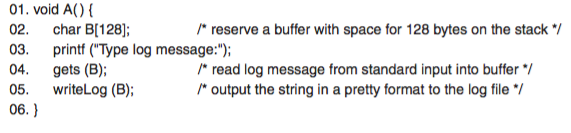
\includegraphics[scale=0.5]{imagenes/buffer-overflow}


El problema con esta función es que la función \textit{gets} lée caracteres de la entrada estándar hasta encontrar un caracter de nueva línea, por lo tanto, si el usuario ingresa 256 caracteres, los 128 caracteres restantes se escribirán en el stack, pisando todo lo que había antes.

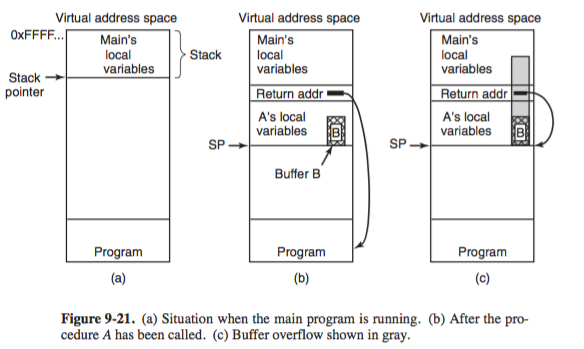
\includegraphics[scale=0.6]{imagenes/buffer-overflow2}

Las consecuencias de esto son que un atacante puede sobreescribir el return address de la función, y hacer que el flujo de instrucciones salte al código malicioso del atacante. Comunmente, el código del atacante es usado para lanzar una shell (mediante la syscall \textit{exec}) y de esta forma tomar control del sistema.

Existen distintas técnicas que se utilizan como defensa.

\subsubsection{Stack Canaries}

La idea es que el compilador inserta un valor aleatorio en el stack (el canary), justo debajo de la dirección de retorno. Al momento de retornar de la función, el compilador inserta código para chequear el valor del canary. Si el valor cambió, el programa termina. Sin embargo, hay maneras de saltearse el canary y sobreescribir el valor de retorno directamente.

\subsubsection{Data Execution Prevention}

La idea de este método es prohibir que se ejecute código en el stack o en el heap. Para lograr esto se provee soporte desde el hardware con el bit NX (no Execute). Los ataques de inyección de código ya no funcionarán si el código provisto por el atacante no se puede ejecutar.

\subsubsection{ASLR}

ASLR (Address Space Layout Randomization) consiste en aleatorizar las direcciones de memoria en donde se van a correr los procesos, para desincentivar atauqes en donde haya saltos a direcciones específicas de memoria.

\subsubsection{Format Strings}

Consideremos el siguiente programa:

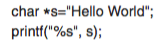
\includegraphics[scale=0.7]{imagenes/format-string1}

Este programa es correcto. Sin embargo, si el programador escribe:

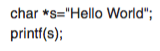
\includegraphics[scale=0.7]{imagenes/format-string2}

hay un problema grave. \textit{printf} toma un número variable de argumentos, y el parámetro $s$ no es simplemente un string, es un \textit{format string}. Hay algunos indicadores de formato que sólo formatean la salida, como $\%s$ y $\%d$, hay otros como $\%n$ que no imprimen nada. En vez de eso, calcula cuántos caracteres deberían ya haberse imprimido en el lugar en el que está del string y guarda ese valor en el argumento de \textit{printf}

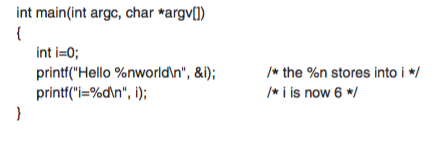
\includegraphics[scale=0.7]{imagenes/format-string3}

En este caso se modifica la variable $i$ al llamar a \textit{printf}, algo que no es tan obvio. Es decir, esta llamada a \textit{printf} modifica la memoria. Por lo tanto, tenemos una manera de escribir lo que queramos en la memoria.


\subsubsection{Race Conditions}

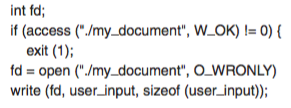
\includegraphics[scale=0.7]{imagenes/race-condition}

Asumimos que el programa tiene SETUID root y que el atacante quiere usar sus privilegios para escribir el archivo de passwords. Lo primero a notar es que no se supone que el programa deba escribir el archivo de passwords; solamente quiere escribir el archivo "my_document". Sin embargo, eso no quiere decir que el usuario tiene permisos para escribir ese archivo. Por ejemplo, el archivo podría ser un link simbólico a otro archivo que no pertenece al usuario, por ejemplo, el archivo de passwords.

Para prevenir esto, el programa hace un chequeo para asegurarse de que el usuario tiene privilegios para escribir el archivo mediante la syscall \textit{access}. La llamada chequea el archivo, devolviendo $0$ si le está permitido el acceso y $-1$ en caso contrario. 

El problema con este programa es que el momento en el que se chequean los privilegios de acceso y el momento en el que se usan los privilegios no es el mismo. Asumamos que una fracción de segundo después del chequeo hecho por \textit{access}, el atacante consigue crear un link simbólico con el mismo nombre de archivo al archivo de passwords. En ese caso, \textit{open} abrirá el archivo incorrecto, y las escrituras del atacante terminarán en el archivo de passwords. Para conseguir esto, el atacante debe crear el link simbólico en el momento exacto. Este ataque es conocido como \textbf{TOCTOU} (Time of Check to Time of Use).

La syscall \textit{access} simplement no es segura. Una manera de solucionar sería abrir el archivo primero, y luego chequear los permisos usando el descriptor del archivo (usando la función \textit{fstat}).



\newpage
\section{Sistemas Distribuídos}

\subsection{Atomicidad}
\subsubsection{Two-phase commit}

Permite a todos los nodos de un sistema distribuído ponerse de acuerdo para hacer un commit a una transacción. El protocolo funciona de la siguiente manera: un nodo es designado como coordinador, y el resto de los nodos son designados como participantes. El protocolo asume que hay almacenamiento estable en cada nodo con un sistema de log write-ahead, que los nodos no están siempre caídos, etc.

\subsubsection{Fase de petición del commit}

\begin{enumerate}[1]
\item El coordinador envía un mensaje "consulta para commit" a todos los participantes.
\item Los participantes ejecutan la transacción hasta el punto donde serán preguntados para realizar el commit.
\item Cada participante responde con un mensaje "acuerdo" si la transacción tuvo éxito, o "abortar" en caso contrario.
\item El coordinador espera hasta que tenga un mensaje de cada participante.
\end{enumerate}


\subsubsection{Fase commit}
\underline{\textbf{Éxito}}

Si el coordinador recibe un mensaje de acuerdo de todos los participantes durante la fase de ptición de commit:

\begin{enumerate}[1]
\item El coordinador envía un mensaje commit a todos los participantes
\item Cada participante completa la operación y libera todos los recursos mantenidos durante la transacción.
\item Todos los participantes envían un ACK al coordinador.
\item El coordinador completa la transacción cuando recibe todos los ACK.
\end{enumerate}

\underline{\textbf{Fracaso}}

Si algún participante envió un mensaje "abortar" durante la fase de petición de commit:

\begin{enumerate}[1]
\item El coordinador envía un mensaje rollback a todos los participantes.
\item Cada participante deshace la transacción usando el log undo y libera todos los recursos.
\item Cada participante envía un ACK al coordinador.
\item El coordinador completa la transacción cuando ha recibido todos los ACK.
\end{enumerate}


La mayor desventaja del protocolo es que es bloqueante. Si el coordinador falla permanentemente, algunos participantes nunca resolverán sus transacciones.

Como las transacciones se guardan en almacenamiento estable, si uno de los nodos se cae temporalmente es posible continuar luego con la transacción cuando el nodo se recupera.


\section{Exclusión Mutua}
\subsubsection{Algoritmo de la panadería}

- Arreglo de tickets y arreglo choosing para sacar ticket

- El thread $i$ pone choosing[i] = true y saca ticket (máximo ticket anterior + 1). Luego choosing[i] = false

- Para cada thread espera:

\quad - Que todos los threads anteriores saquen su ticket

\quad - Que todos los threads con número de ticket menor salgan de su sección crítica. Si hay un thread con el mismo nro. de ticket, desempata por número de thread. 


\newpage
\section{Bibliograf\'ia}
\begin{itemize}
 \item Computer Organization and Architecture, Stallings (8th Edition): Cap\'itulos 4, 17 y 18.
 
 \item Inside the Machine, Stokes: Cap\'itulos 3 y 4.

 \item Clases te\'oricas de Furfaro.
\end{itemize}

\end{document}
